\chapter{Documentazione sperimentale}
\label{app:documentazione}

Si riporta la documentazione sperimentale fornita dal produttore \textit{La Rete Srl}, sulla quale si fondano la caratterizzazione meccanica delle funi e il confronto presentato al \cref{sec:risultati}. I documenti sono riprodotti nella forma in cui sono stati ricevuti.

\section{Prove quasi statiche sulla rete}
\label{app:prove_quasi_statiche}

I diagrammi forza-spostamento riportati di seguito costituiscono il riferimento sperimentale del \cref{sec:risultati}. Le curve impiegate nei confronti sono state ottenute per digitalizzazione di tali diagrammi e normalizzate sullo spostamento finale dichiarato nel prospetto riassuntivo.

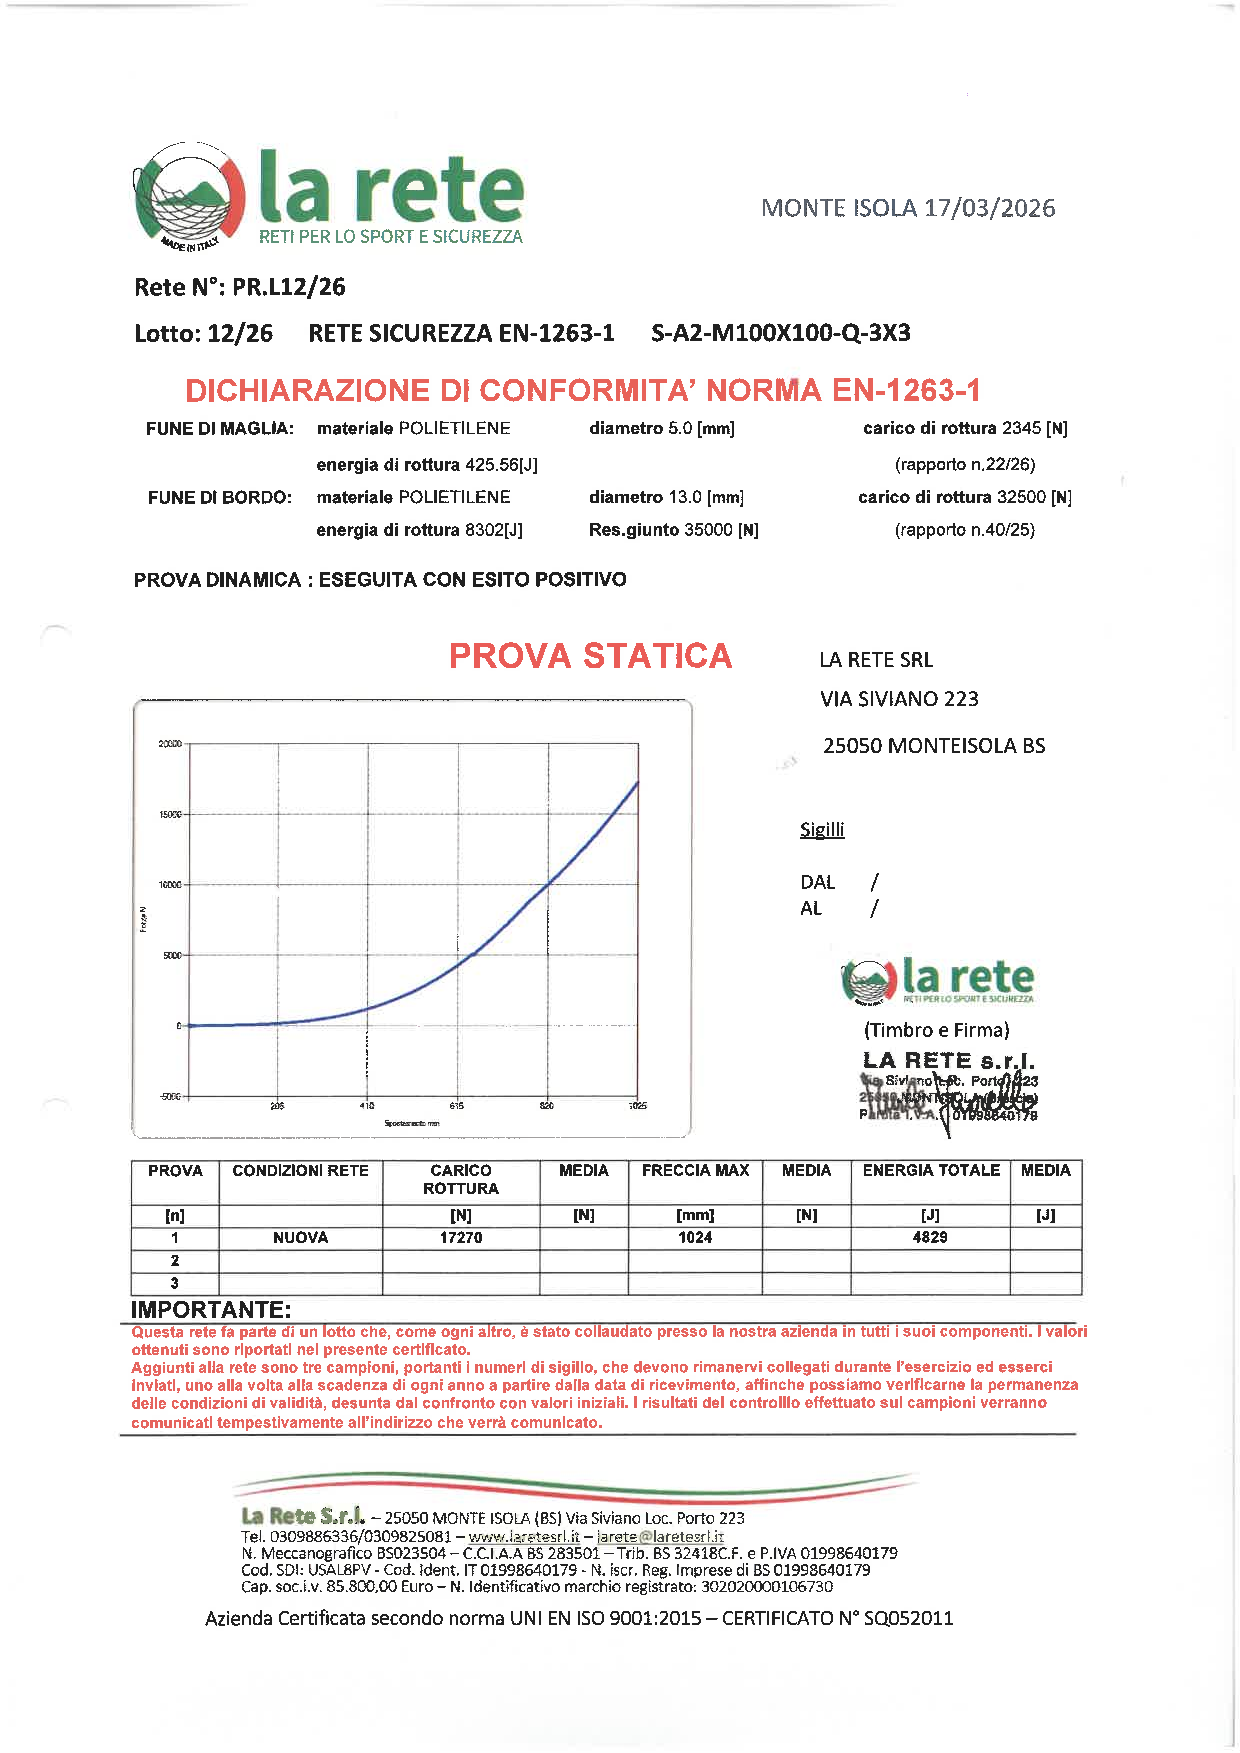
\includepdf[pages=1, scale=0.88, offset=0 -45pt,
            pagecommand={\subsection{Rete a maglia \texorpdfstring{$100\times100$}{100x100}}\thispagestyle{plain}}]
           {141_appendici/certificato_100x100.pdf}

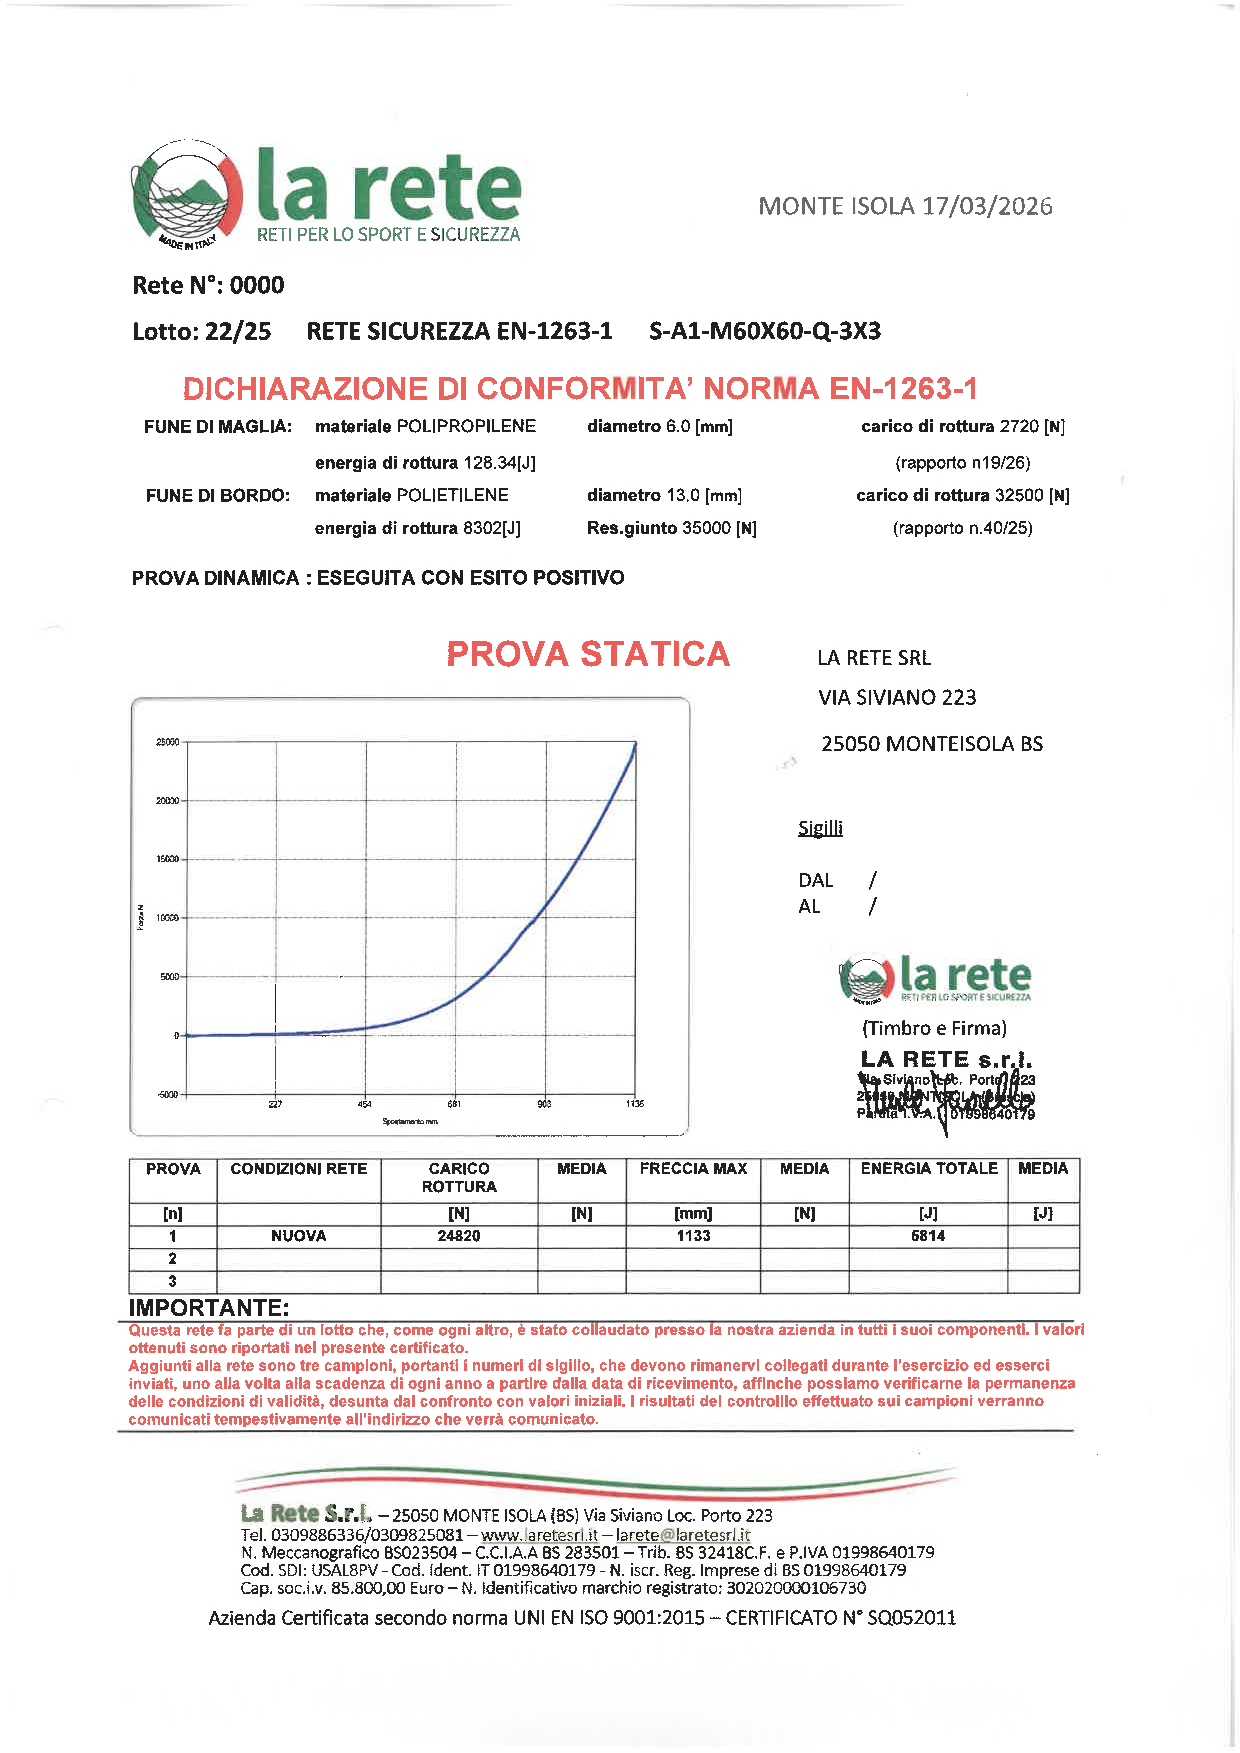
\includepdf[pages=1, scale=0.88, offset=0 -45pt,
            pagecommand={\subsection{Rete a maglia \texorpdfstring{$60\times60$}{60x60}}\thispagestyle{plain}}]
           {141_appendici/certificato_60x60.pdf}

\section{Prove di trazione sulla singola maglia}
\label{app:prove_trazione}

I rapporti di prova a trazione sulla singola maglia, eseguiti secondo la \cite{ENISO1806-2002}, costituiscono l'input della caratterizzazione meccanica degli elementi di cui alla \cref{sec:caratterizzazione_funi}. Di ciascun rapporto si riproducono il prospetto riassuntivo e il diagramma forza-allungamento. La linearizzazione a tratti della \cref{sec:linearizzazione} non è stata tuttavia dedotta da tali diagrammi, bensì dalla serie numerica allegata a ciascun rapporto ed estratta dai file in formato \texttt{.xls} forniti dal produttore, che per ragioni di spazio non viene qui riprodotta.

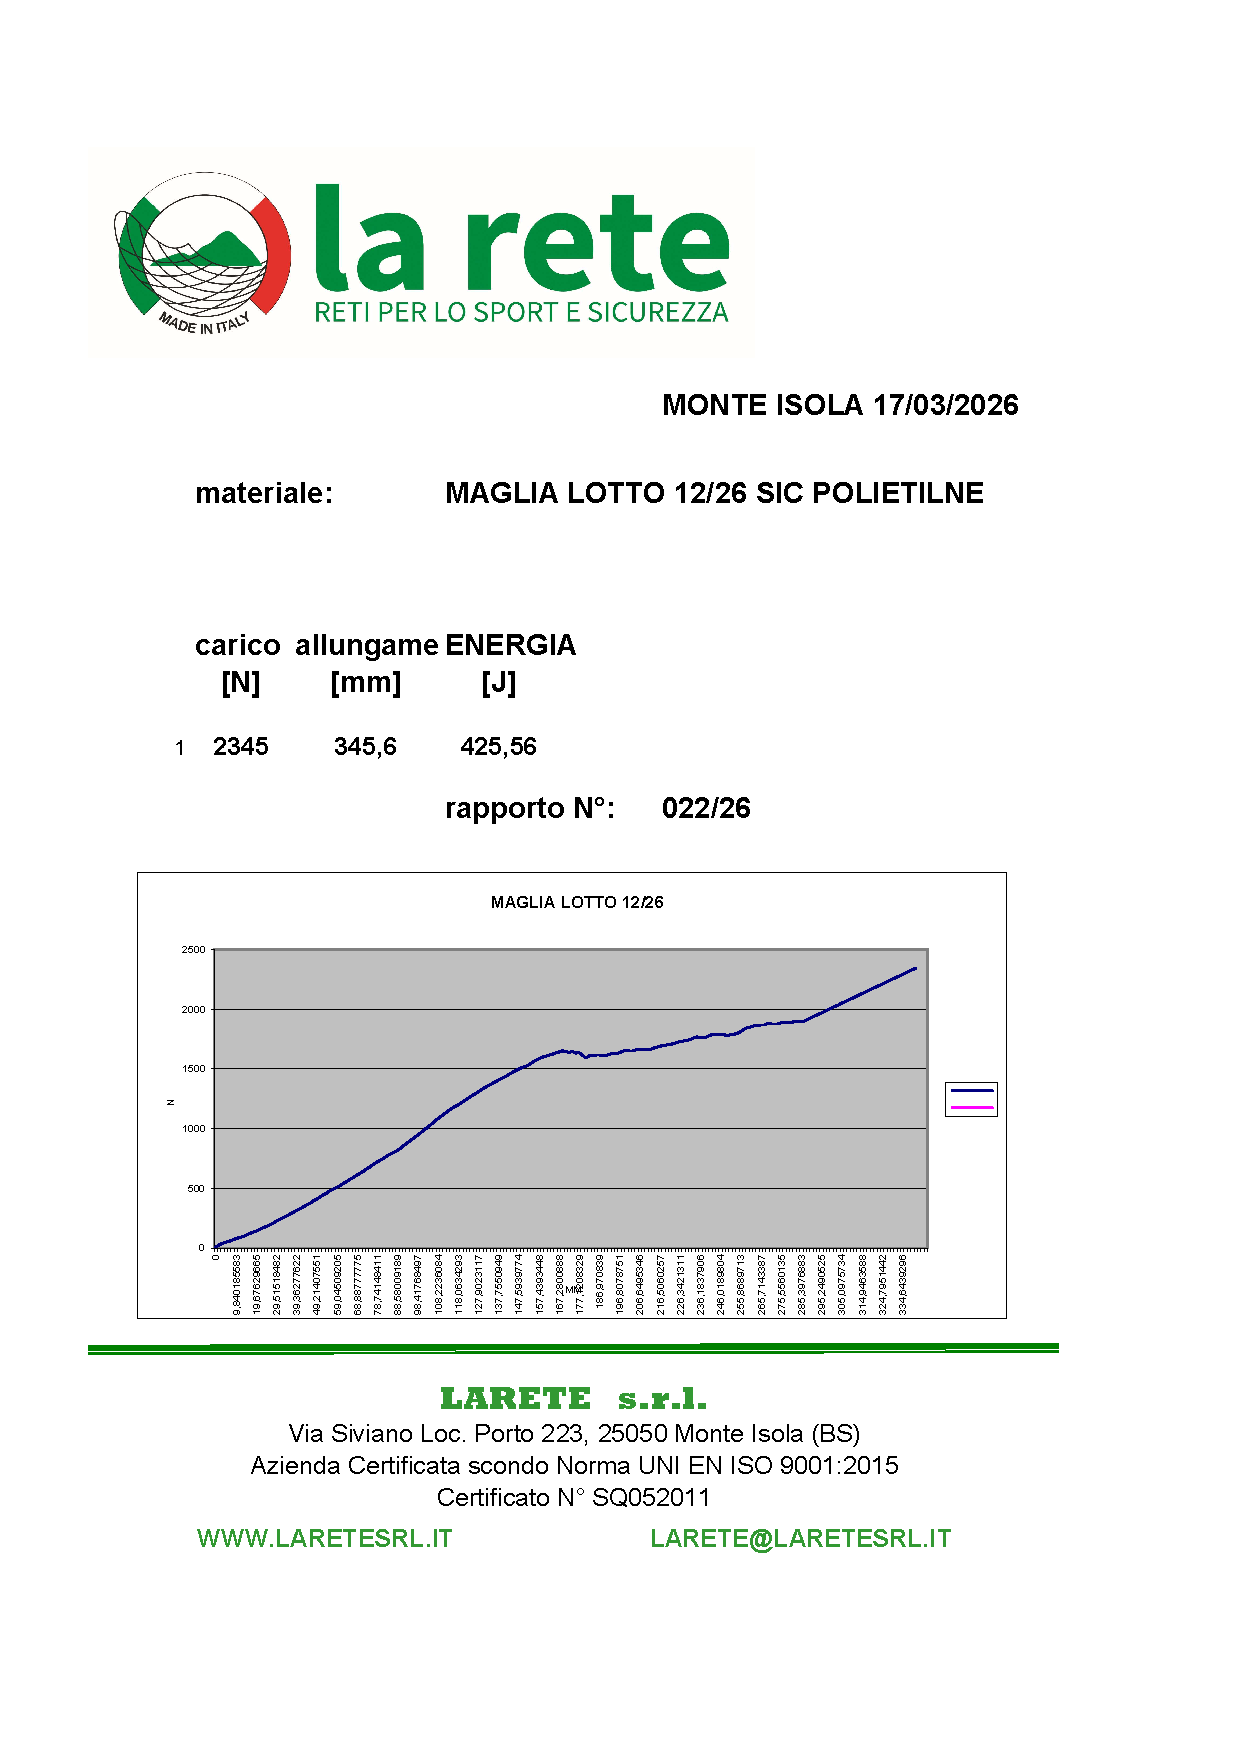
\includepdf[pages=1, scale=0.88, offset=0 -35pt,
            pagecommand={\subsection{Rapporto di prova n.~022 --- maglia \texorpdfstring{$100\times100$}{100x100}}\thispagestyle{plain}}]
           {141_appendici/rapporto_022_100x100.pdf}

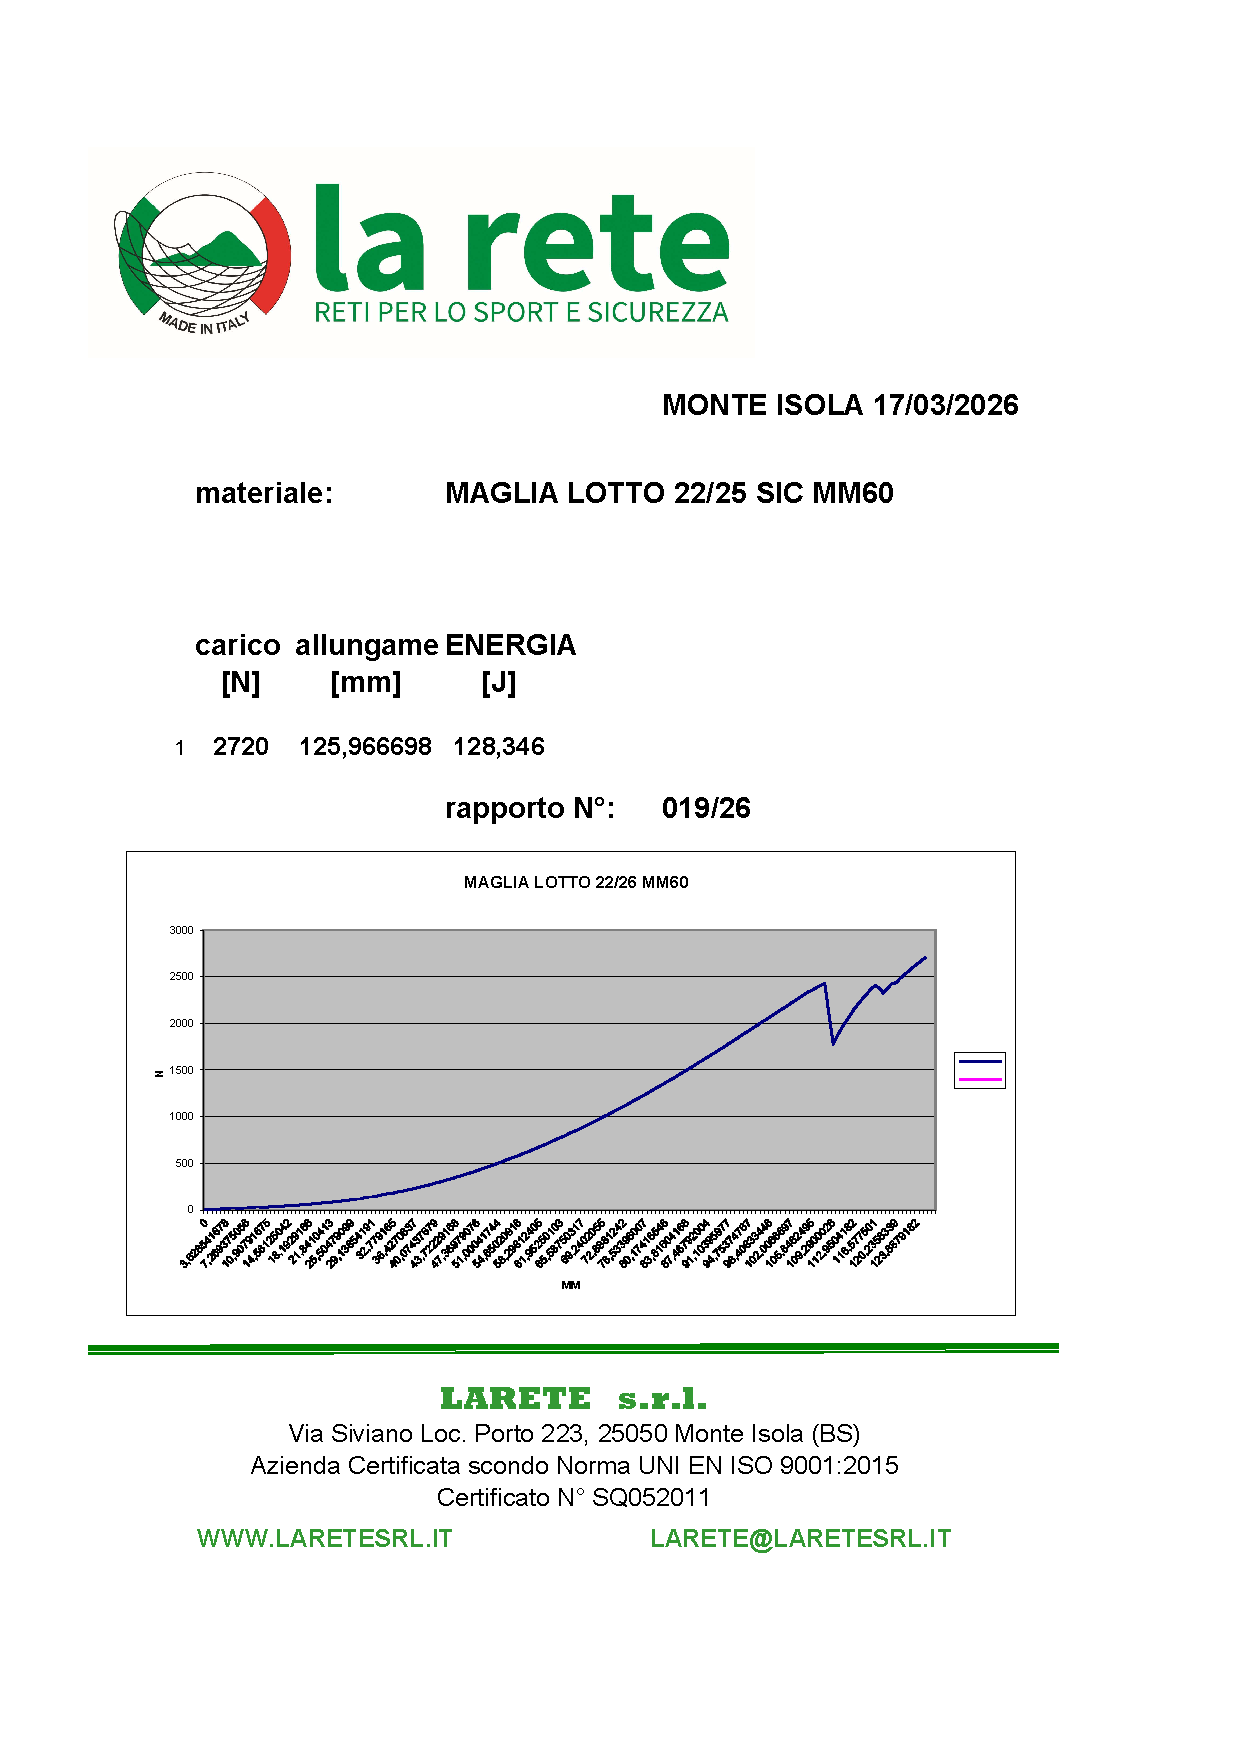
\includepdf[pages=1, scale=0.88, offset=0 -35pt,
            pagecommand={\subsection{Rapporto di prova n.~019 --- maglia \texorpdfstring{$60\times60$}{100x100}}\thispagestyle{plain}}]
           {141_appendici/rapporto_019_60x60.pdf}